\section{Results}
    \subsection{Classification}
		Following are the results for the SGD algorithm applied to the credit card data set. Figure \ref{fig:SGDacc} illustrates the accuracy scores of the SGD algorithm using a hyperparameter and learning rate grid search.
		\begin{figure}[H]
			\centering
			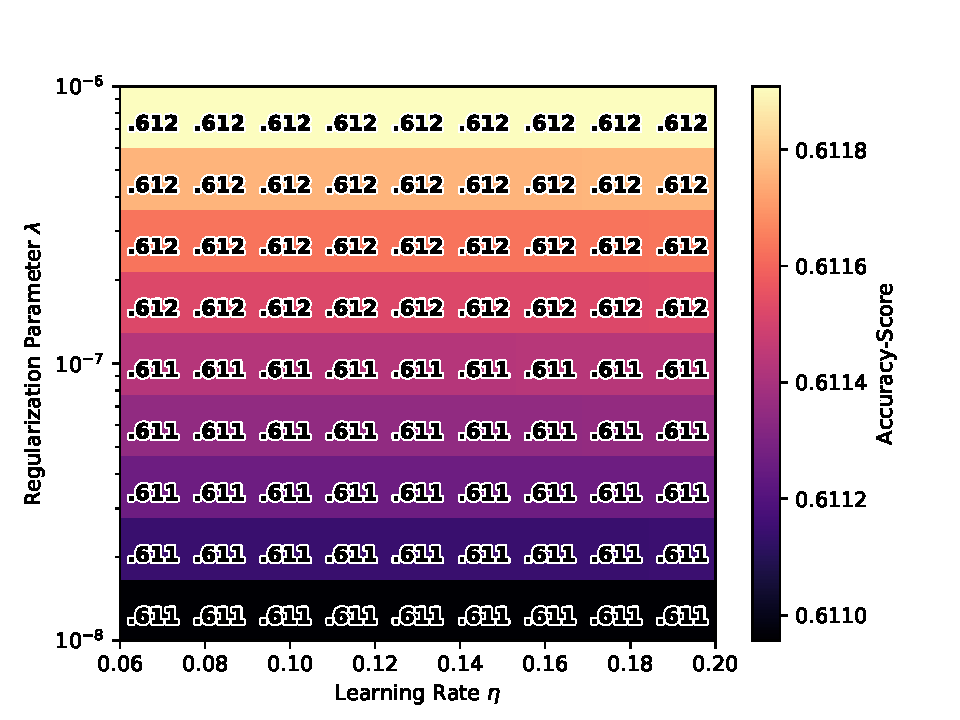
\includegraphics[width=0.45\textwidth]{figures/SGD_acc.pdf}
			\caption{The accuracy scores of the SGD algorithm for different $\eta$ and $\lambda$ values. The maximum accuracy score of the array is $0.612$, using $\lambda=10^{-6}$}
			\label{fig:SGDacc}
		\end{figure}
		Figure \ref{fig:SGDf1} illustrates the F1 scores of the SGD algorithm using a hyperparameter and learning rate grid search.
		\begin{figure}[H]
			\centering
			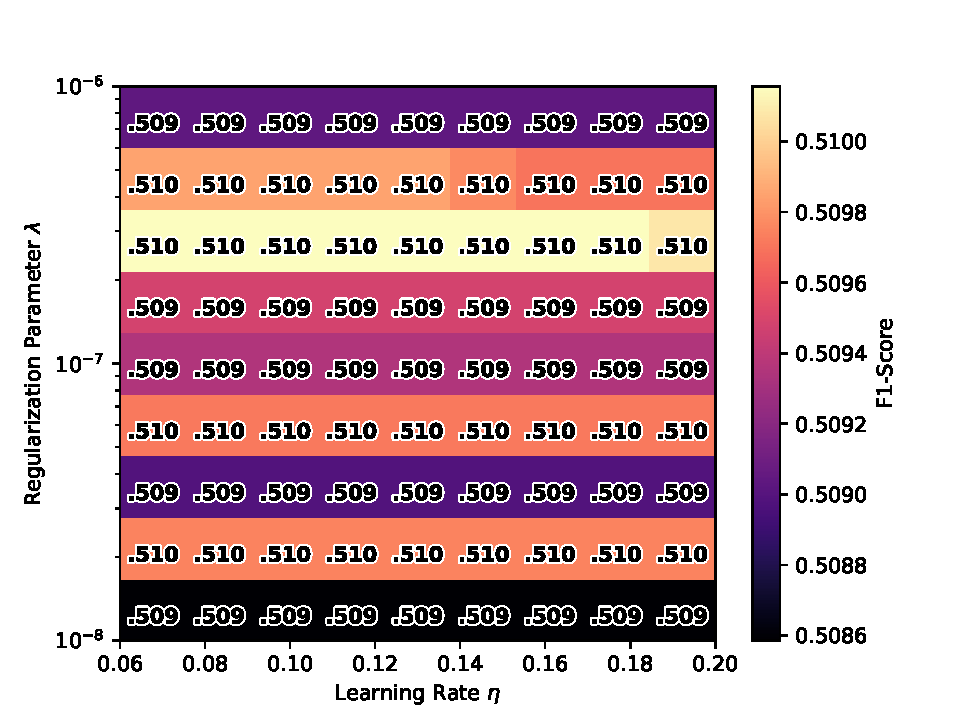
\includegraphics[width=0.45\textwidth]{figures/SGD_F1.pdf}
			\caption{The F1 scores of the SGD algorithm for different $\eta$ and $\lambda$ values. The maximum F1 score of the array is $0.510$, using $\lambda=3.594\cdot10^{-7}$}
			\label{fig:SGDf1}
		\end{figure}
		Figure \ref{fig:SGDauc} illustrates the AUC scores of the SGD algorithm using a hyperparameter and learning rate grid search.
		\begin{figure}[H]
			\centering
			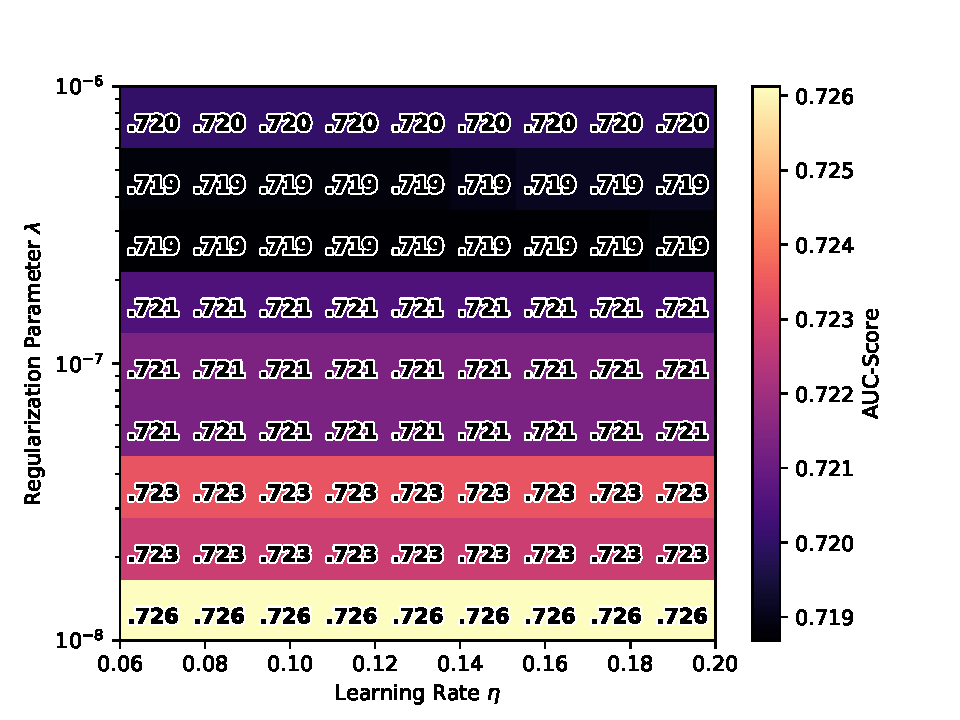
\includegraphics[width=0.45\textwidth]{figures/SGD_AUC.pdf}
			\caption{The AUC scores of the SGD algorithm for different $\eta$ and $\lambda$ values. The maximum accuracy score of the array is $0.726$, using $\lambda=10^{-8}$}
			\label{fig:SGDauc}
		\end{figure}
		Figure \ref{fig:SGDgs} illustrates the gains ratios of the SGD algorithm using a hyperparameter and learning rate grid search.
		\begin{figure}[H]
			\centering
			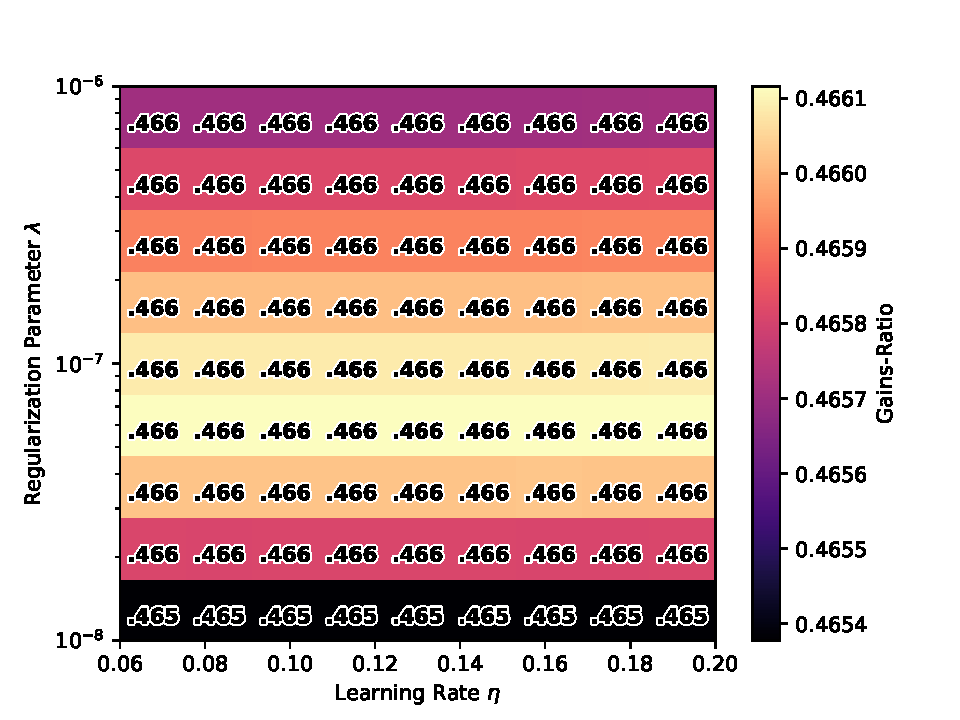
\includegraphics[width=0.45\textwidth]{figures/SGD_gains.pdf}
			\caption{The gains ratios of the SGD algorithm for different $\eta$ and $\lambda$ values. The maximum accuracy score of the array is $0.466$, using $\lambda=4.642\cdot 10^{-8}$}
			\label{fig:SGDgs}
		\end{figure}
		Following are the results from the ANN study of the credit card data. The accuracy scores of the neural network hyperparameter and learning rate grid search are illustrated in figure \ref{fig:cc_acc}.
		\begin{figure}[H]
			\centering
			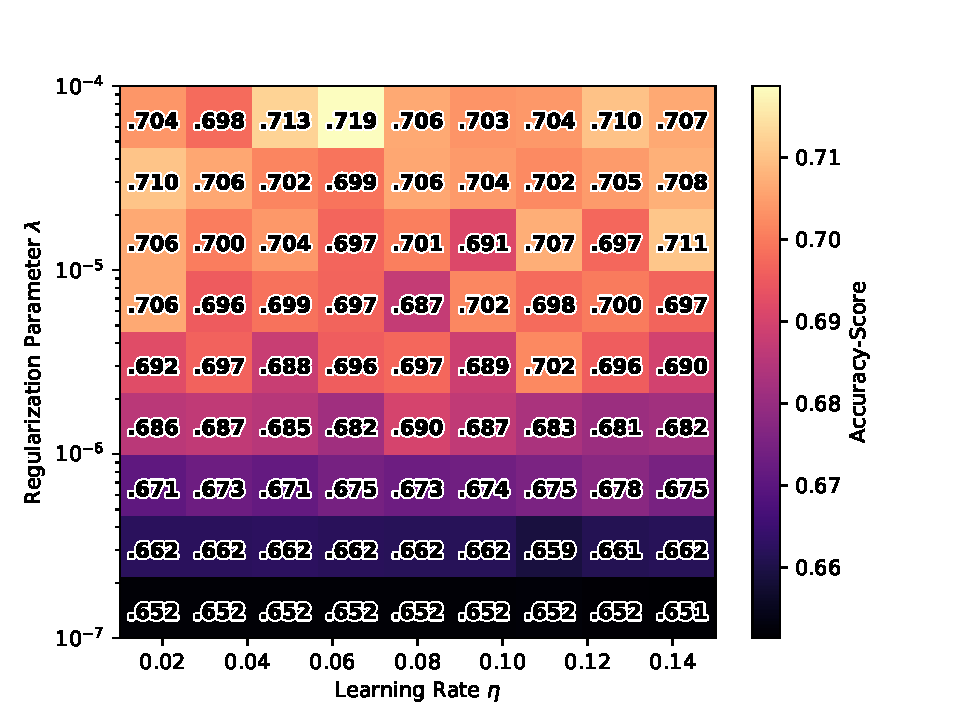
\includegraphics[width=0.45\textwidth]{figures/cc_res_0.pdf}
			\caption{The accuracy score of the classification neural network for different $\eta$ and $\lambda$ values. The maximum accuracy score of the array is $0.719$, using $\eta=0.056$ and $\lambda=10^{-4}$}
			\label{fig:cc_acc}
		\end{figure}
		The F1-scores of the neural network hyperparameter and learning rate grid search are illustrated in figure \ref{fig:cc_F1}.
		\begin{figure}[H]
			\centering
			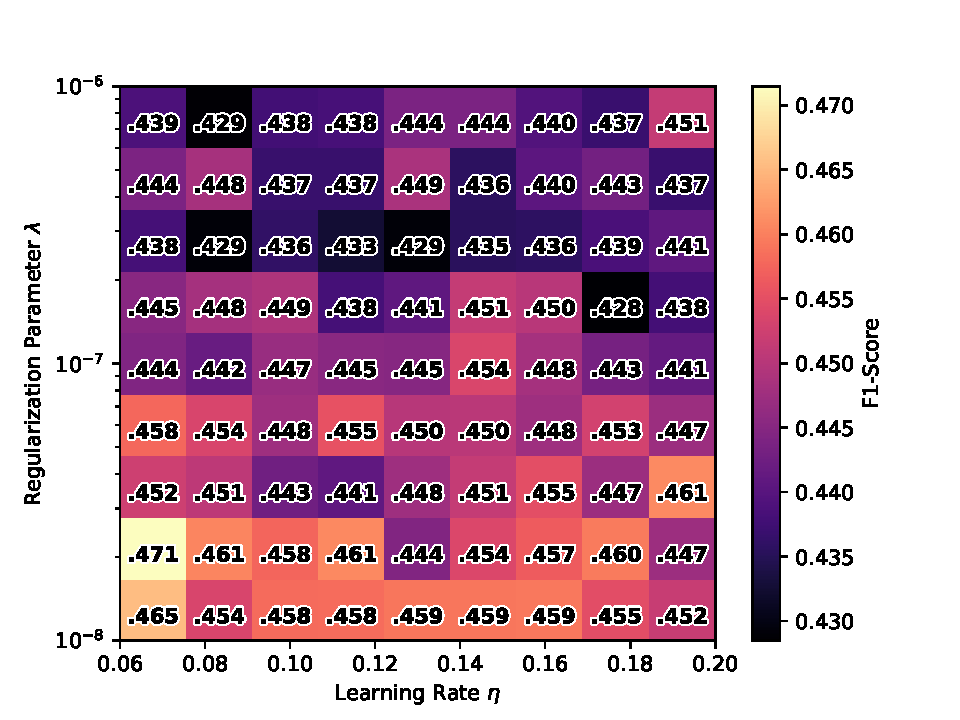
\includegraphics[width=0.45\textwidth]{figures/cc_res_1.pdf}
			\caption{The F1 score of the classification neural network for different $\eta$ and $\lambda$ values. The maximum F1 score of the array is $0.484$, using $\eta=0.103$ and $\lambda=10^{-7}$}
			\label{fig:cc_F1}
		\end{figure}
		The AUC-scores of the neural network hyperparameter and learning rate grid search are illustrated in figure \ref{fig:cc_auc}.
		\begin{figure}[H]
			\centering
			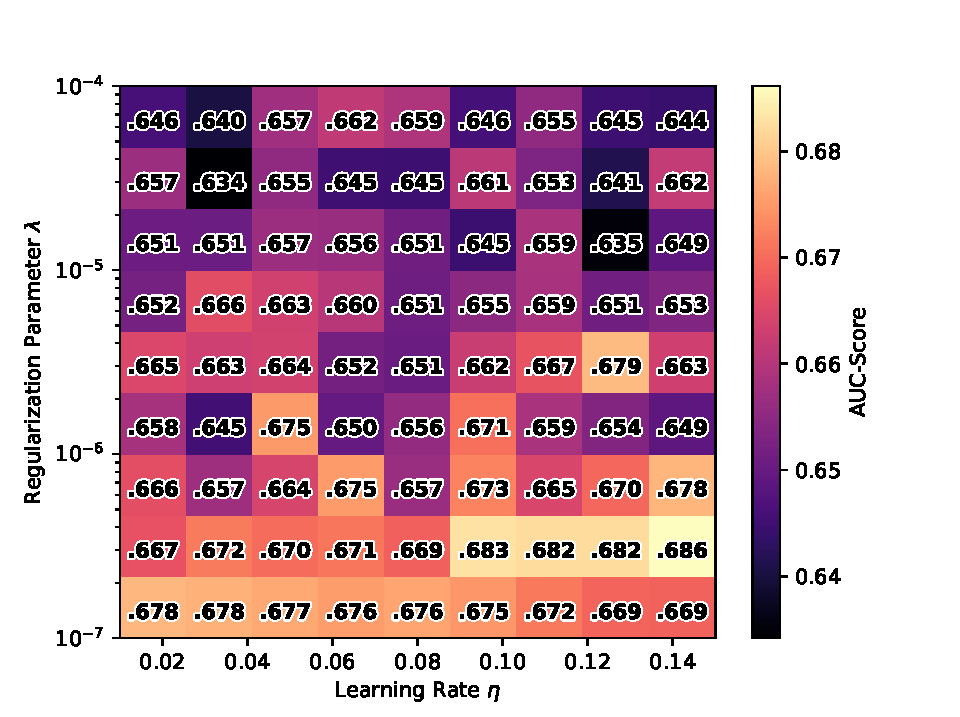
\includegraphics[width=0.45\textwidth]{figures/cc_res_2.pdf}
			\caption{The AUC-score of the classification neural network for different $\eta$ and $\lambda$ values. The maximum AUC-score of the array is $0.686$, using $\eta=0.150$ and $\lambda=2.154\cdot 10^{-7}$}
			\label{fig:cc_auc}
		\end{figure}
		The gains-ratio of the neural network hyperparameter and learning rate grid search are illustrated in figure \ref{fig:cc_gr}.
		\begin{figure}[H]
			\centering
			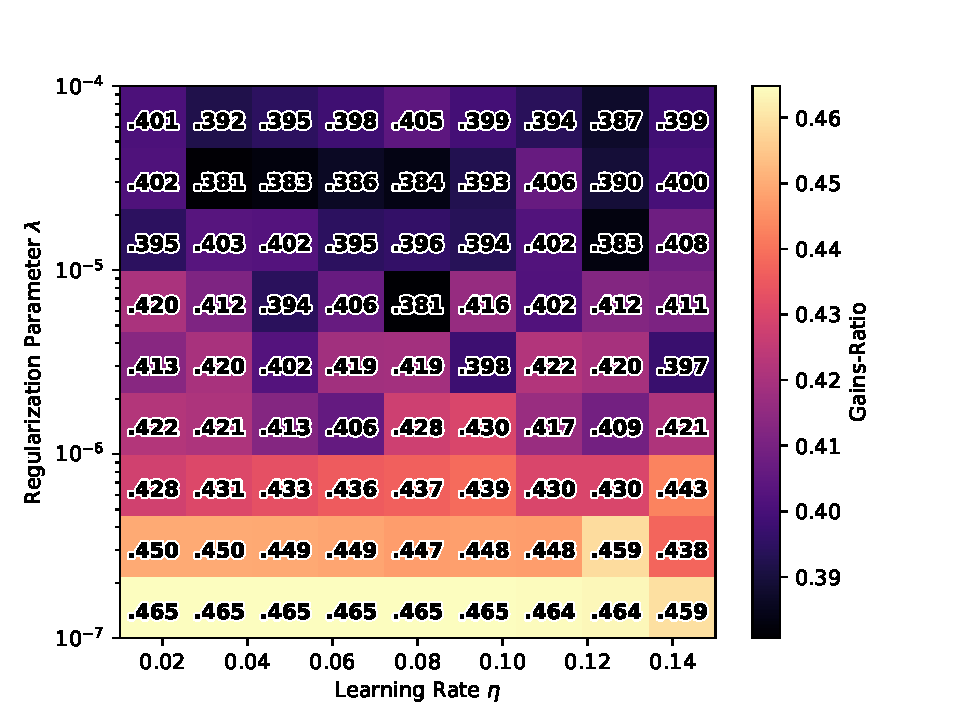
\includegraphics[width=0.45\textwidth]{figures/cc_res_3.pdf}
			\caption{The gains-ratio of the classification neural network for different $\eta$ and $\lambda$ values. The maximum gains-ratio of the array is $0.465$, using $\eta \in [0.010, 0.103]$ and $\lambda=10^{-7}$}
			\label{fig:cc_gr}
		\end{figure}
    \subsection{Regression}
    	Following are the results of the Ridge scheme applied to Franke's function. These results are the ones produced in project 1 \cite{4}. Table \ref{tab:conclusion_table_Frankes} lists the results of the comparison of the three methods of regression on Franke's function.
    	\begin{table}[H]
    		\centering
    		\begin{tabular}[t]{l@{\hskip 0.3in}c@{\hskip 0.3in}c@{\hskip 0.2in}c}
    			\toprule
    			Scheme & MSE minimum & $p_{deg}$ & $\log(\lambda)$ \\
    			\midrule
    			Ridge & $2\times 10^{-4}$ & 9 & -16\\
    			\bottomrule
    		\end{tabular}
	    	\caption{Table listing the final results and comparisons of the regressional methods applied to Franke's function.}
    		\label{tab:conclusion_table_Frankes}
    	\end{table}
    	Following are the results from the ANN study of the data produced by Franke's function. The MSE scores of the neural network hyperparameter and learning rate grid search are illustrated in figure \ref{fig:ff_mse}.
    	\begin{figure}[H]
    		\centering
    		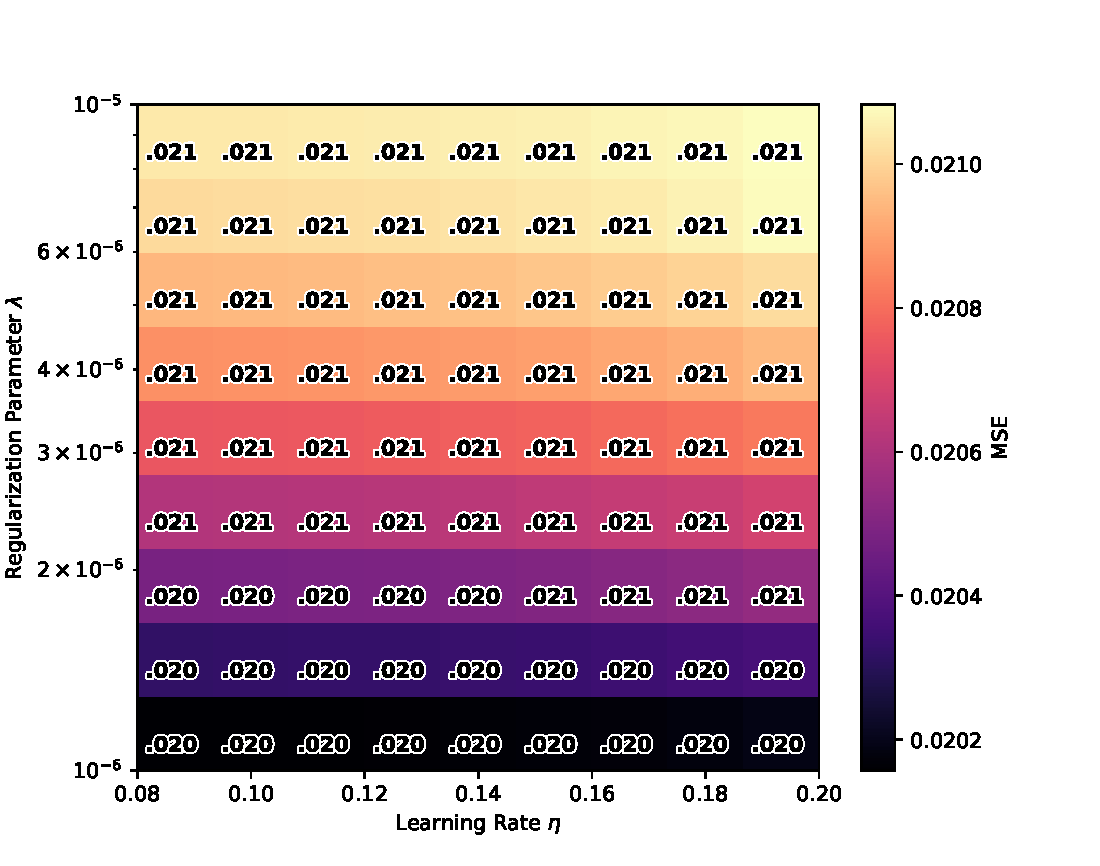
\includegraphics[width=0.45\textwidth]{figures/ff_res_0.pdf}
    		\caption{The MSE scores of the neural network applied to Franke's function for different $\eta$ and $\lambda$ values. The minimum MSE value of the array is 0.20, using $\eta \in [0.08, 0.2]$ and $\lambda=10^{-6}$.}
    		\label{fig:ff_mse}
    	\end{figure}
	    The R2 scores of the neural network hyperparameter and learning rate grid search are illustrated in figure \ref{fig:ff_r2}.
    	\begin{figure}[H]
    		\centering
    		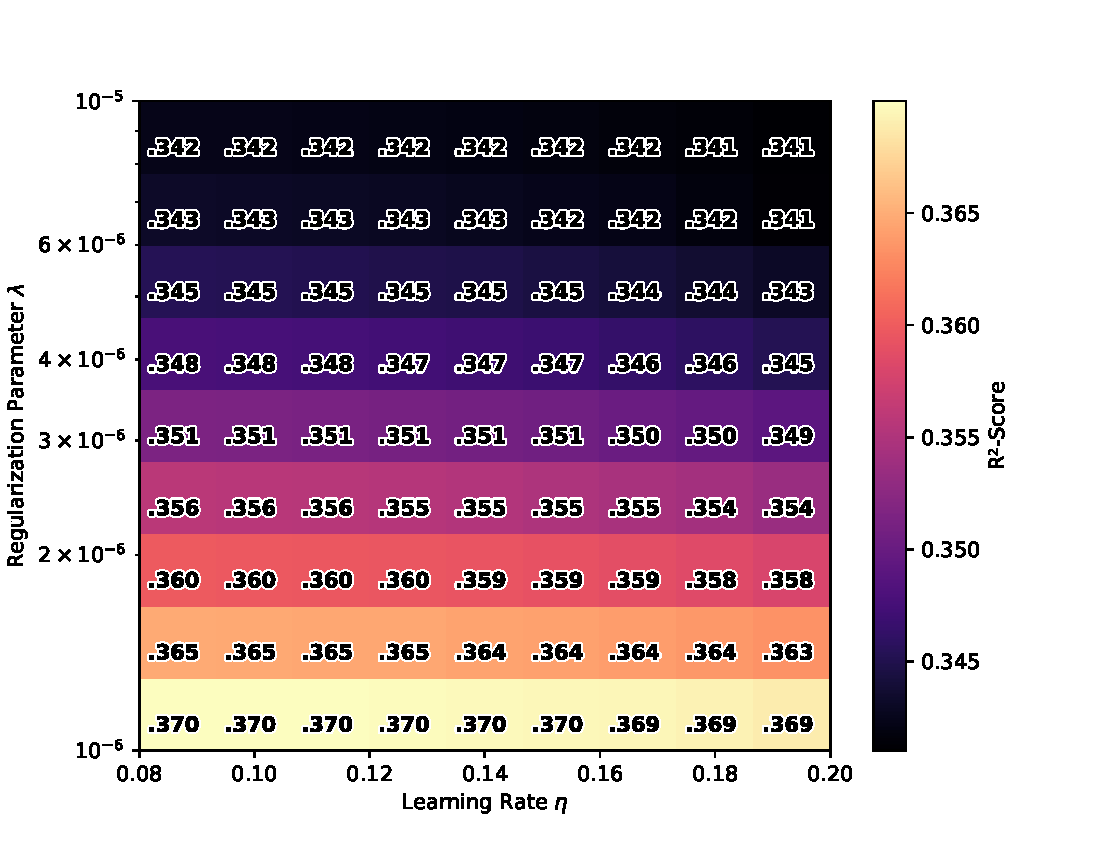
\includegraphics[width=0.45\textwidth]{figures/ff_res_1.pdf}
    		\caption{The R2 scores of the neural network applied to Franke's function for different $\eta$ and $\lambda$ values. The maximum MSE value of the array is 0.37, using $\eta \in [0.08, 0.2]$ and $\lambda=10^{-6}$.}
    		\label{fig:ff_r2}
    	\end{figure}